\documentclass{article}
\usepackage{geometry}
\usepackage{amsmath}
\usepackage{float}
\usepackage{fancybox,graphicx}
\usepackage{xcolor}
\geometry{
    a4paper,
    margin=2.75cm}
\definecolor{gainsboro}{RGB}{240, 240, 240}
    
\title{Tarea 0 EDDA}
\author{Adriana Ramírez Vigueras\\ Marco Antonio Velasco Flores\\ Fhernanda Montserrat Romo Olea}
\date{Fecha de entrega: Martes 5 de Septiembre}

\begin{document}

\maketitle

\begin{enumerate}

\item Tienes la siguiente sucesión elementos $S = \{5,17,6,8,2,4,1,12,10,3,21\}$. Toma los elementos de dicha sucesión únicamente de izquierda a derecha para los siguientes ejercicios, es decir, el primer elemento a extraer será el $5$, luego el $17$, el $6$, etc... (4 puntos)

\begin{enumerate}

    \item Inserta los 5 primeros elementos dentro de una pila. Saca dos veces el elemento al tope de la pila. Mete los siguientes 4 elementos de $S$. Saca otros 2 elementos de la pila. Por último, ingresa un elemento más. Si sacas todos los elementos de la pila restantes, ¿En qué orden salen? (0.5 pts.)

    \item Inserta los 6 primeros elementos dentro de una cola. Saca 4 elementos de la cola. Ingresa todos los elementos restantes de $S$. Saca otros 3 elementos. Si sacas todos los elementos de la cola restantes, ¿En qué orden salen? (0.5 pts.)
    
    \item Construye un árbol binario ordenado con los elementos de $S$ insertándolos conforme éstos son dados (Ojo, no necesitas balancear el árbol). (0.5 pts.)

    \item Dado el árbol anterior. Realiza una rotación en el nodo que contiene al 17 hacia la derecha. (0.5 pts.)

    \item Ahora sobre el árbol resultante anterior. Realiza una rotación en el nodo que contiene al 6 hacia la izquierda. (0.5 pts.)

    \item Realiza un recorrido BFS sobre el árbol resultante anterior. ¿En qué orden son devueltos los elementos? (0.5 pts.)

    \item Realiza 2 recorridos DFS sobre el árbol resultante del ejercicio 5, uno en pre-orden y otro en post-orden. ¿En qué orden son devueltos los elementos en cada caso? (1 pts.)

\end{enumerate}

\item Tenemos dos árboles binarios de búsqueda con O(n) elementos cada uno y queremos construir una lista de tamaño O(2n)  con los elementos de ambos árboles de tal manera que la lista resultante este ordenada de mayor a menor. Diseña un algoritmo de complejidad O(n) para obtener esta lista, justifica la complejidad y explica claramente tu algoritmo con un ejemplo. Nota: Toma en cuenta que el árbol binario de búsqueda puede tener elementos repetidos. (2 puntos)

\item Preparata se encuentra haciendo el programa "X", el programa "X" es un juego para resolver un cubo Rubik, el usuario analiza el estado de  un cubo Rubik en tres dimensiones y con base en su criterio  elije una de las operaciones $a_1 ... a_n$, para modificar el estado del cubo, Preparata sabe que estas operaciones tienen "inversa" es decir si la operación $a_1$ nos lleva del estado $e_1$ al estado $e_2$ entonces la inversa de la operación $a_1$ nos regresa al estado $e_1$, el ya tiene programadas todas las operaciones con sus respectivas operaciones inversas, pero no sabe como implementar la transición y el regreso de los estados para que el usuario pueda hacer una operación o deshacerla, el usuario también puede realizar varias operaciones y deshacerlas todas o una parte de ellas, además si ya deshizo un conjunto de operaciones puede volver a recrearlas sin necesidad de volver a pensar en ellas.
    
El cree que una estructura de datos le podría ayudar con esto. Ayudale a Preparata a descubrir la estructura de datos que necesita y explica detalladamente como  implementar la transición y el regreso de los estados, la complejidad de tu solución debe ser de orden $O(1)$ para deshacer una operación o para recrearla. Nota: Las operaciones tienen orden. (2 puntos)

\item Urrutia esta trabajando en un nuevo proyecto para obtener cuentas de detalle de tablas de información, por ejemplo tenemos las siguientes dos tablas:

\begin{figure}[H]
    \centering
    \shadowsize=0.8pt
    \fboxrule=0pt
    \fboxsep=0pt
    \color{lightgray}
    \shadowbox{\fboxsep=2pt\fcolorbox{gray}{gainsboro}{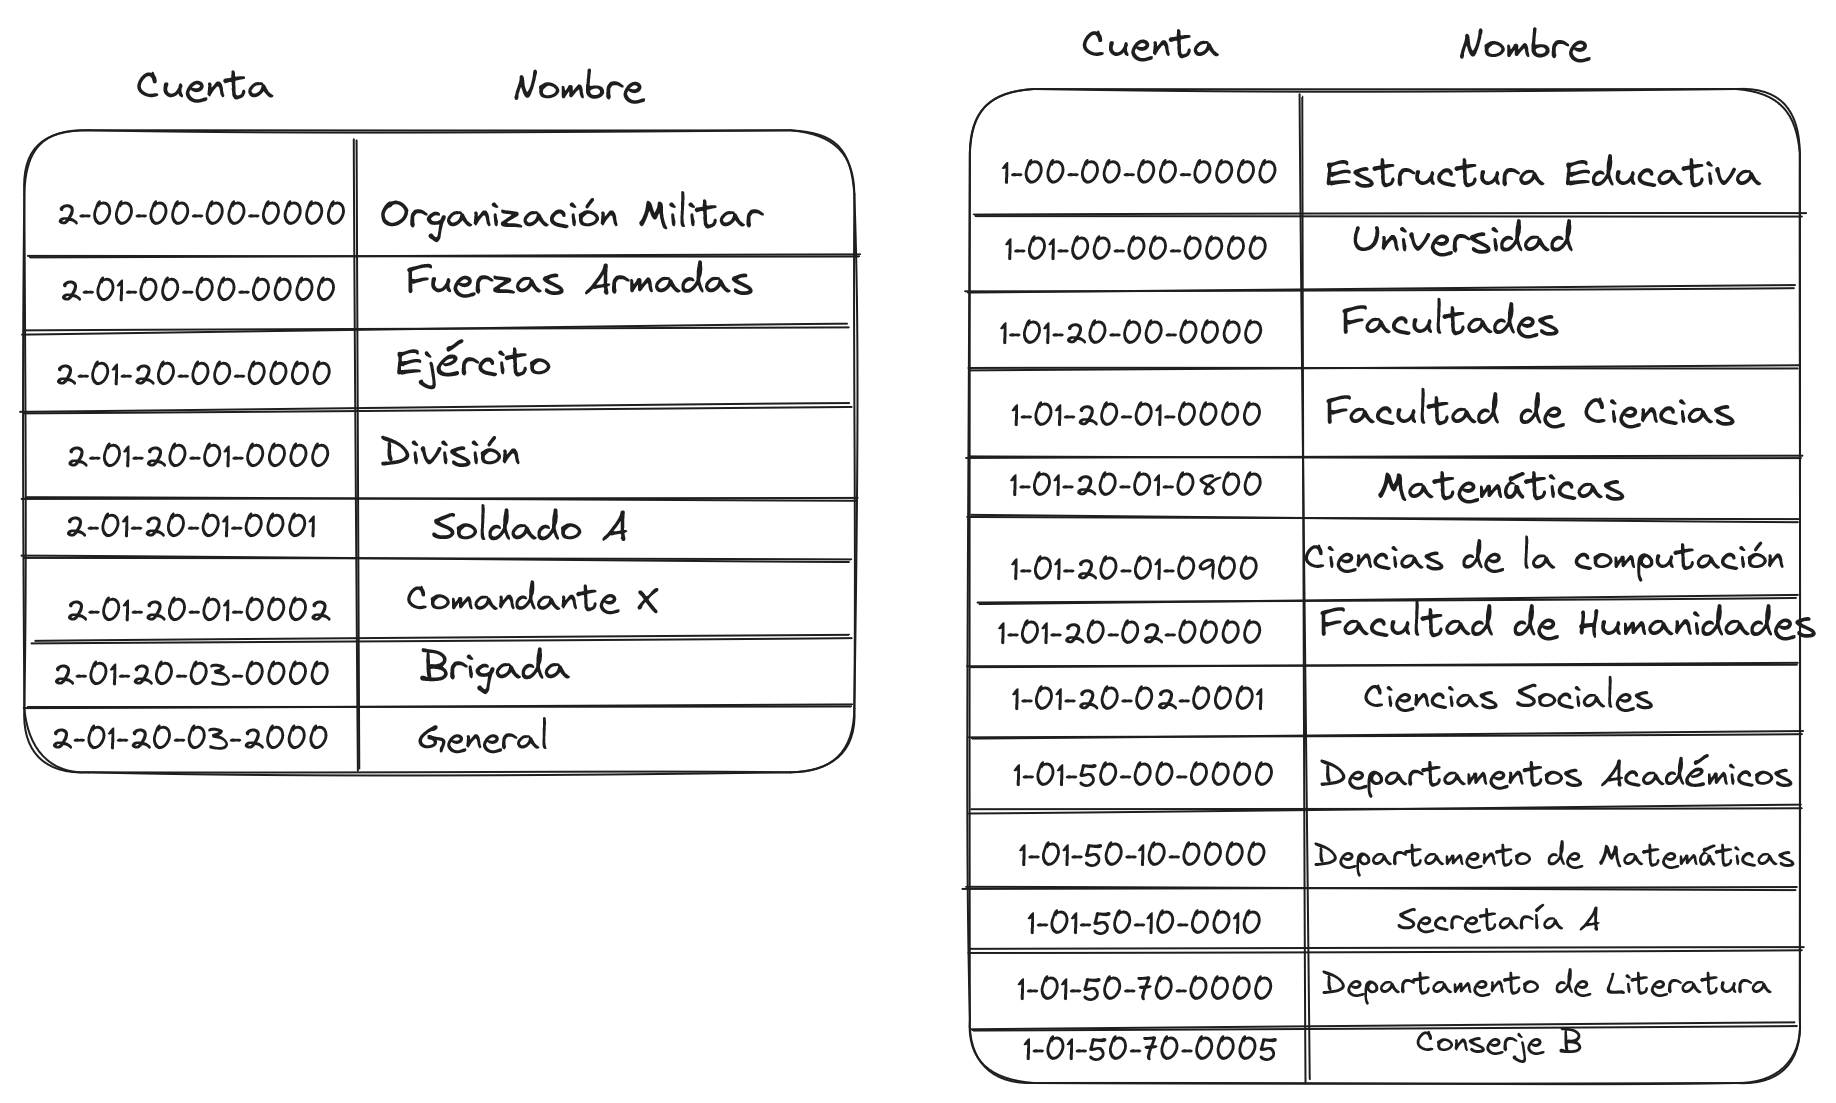
\includegraphics[width=12cm]{Tablas.png}}}
    \color{black}
    \label{fig:12}
\end{figure}
    
Estas tablas contiene información ordenada de formar jerárquica, y a nosotros nos interesaa extraer la información de menor jerarquía pero sin perder el nombre de las cuentas de mayor jerarquía a las que pertenecen, es decir buscamos una tabla como resultado final de esta manera:

\begin{figure}[H]
    \centering
    \shadowsize=0.8pt
    \fboxrule=0pt
    \fboxsep=0pt
    \color{lightgray}
    \shadowbox{\fboxsep=2pt\fcolorbox{gray}{gainsboro}{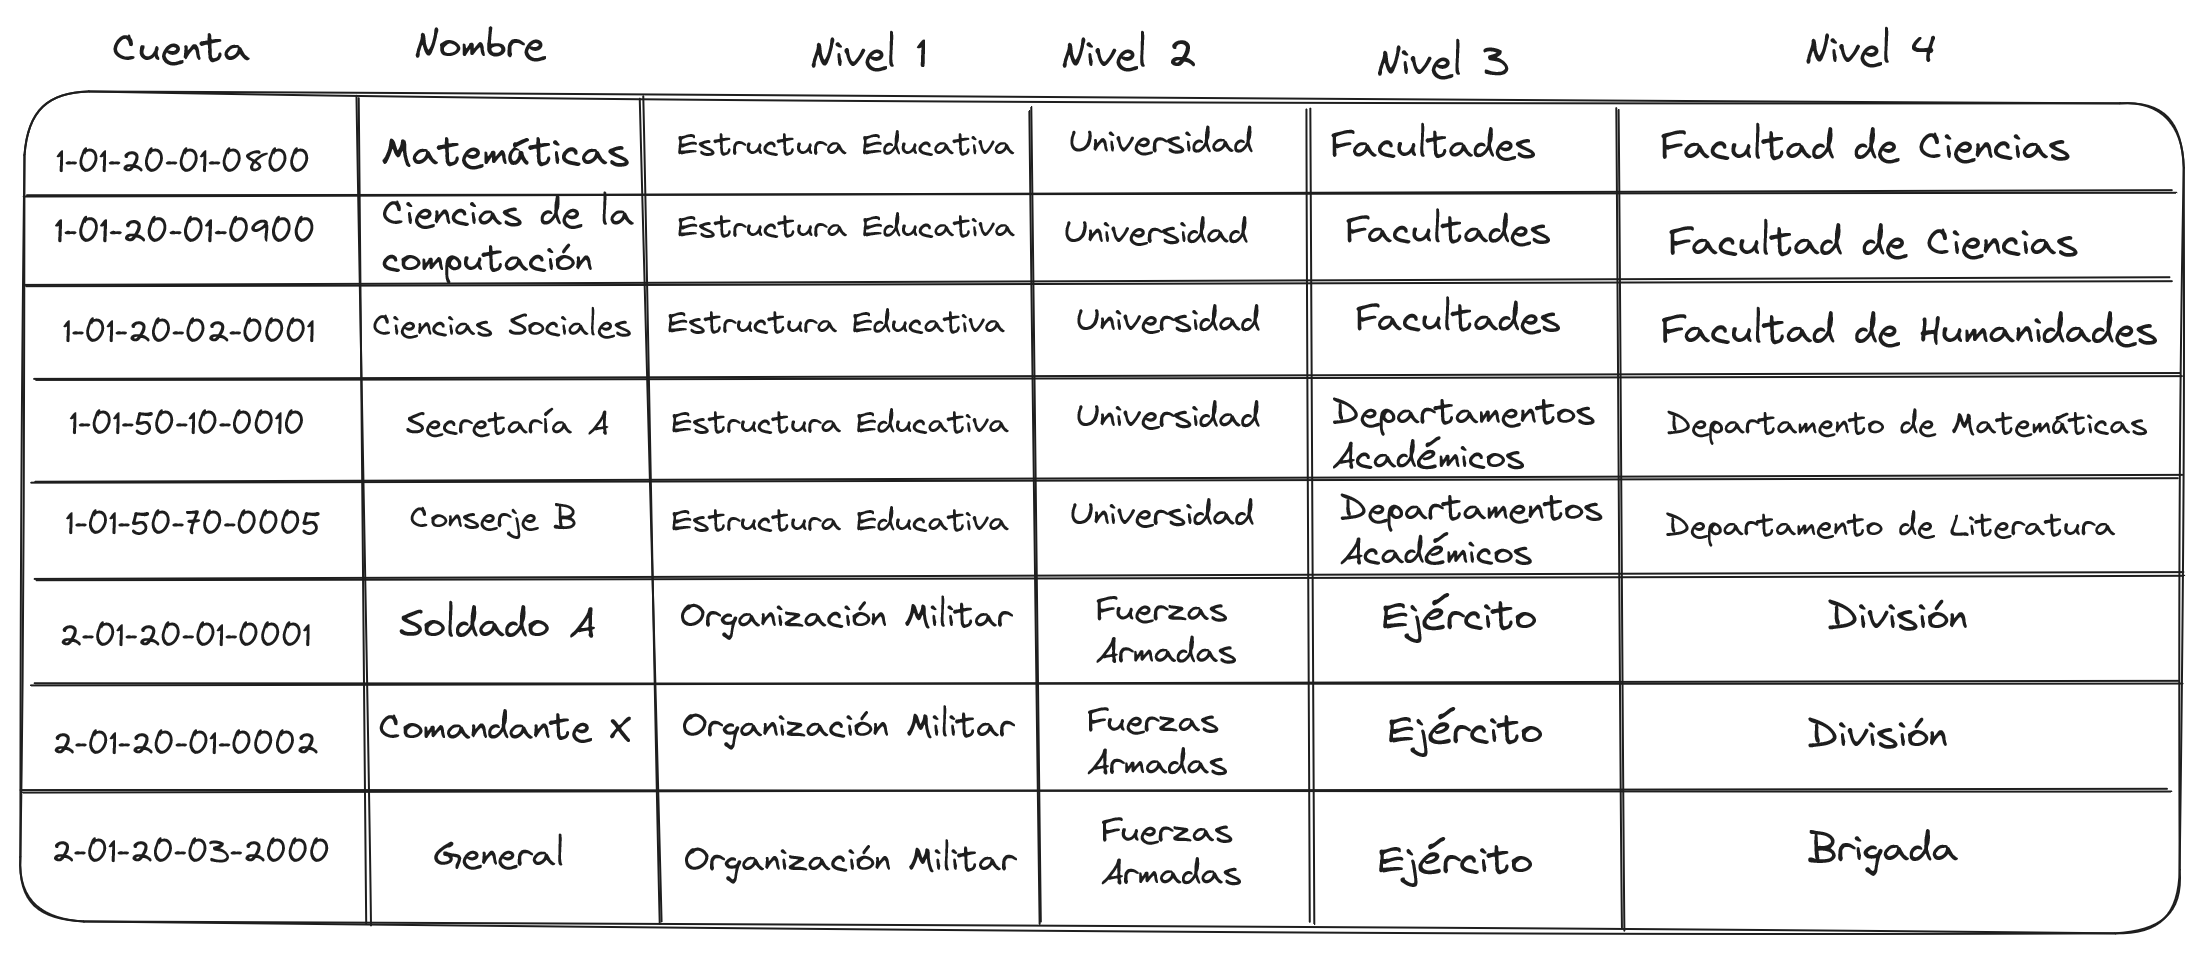
\includegraphics[width=12cm]{Resultado.png}}}
    \color{black}
    \label{fig:12}
\end{figure}

Urrutia se dio cuenta que puede construir un árbol n-ario para resolver de manera fácil este problema basándose en los números de cuenta para construir una llave que le ayudará a decidir si un nodo es hijo o no de otro nodo, hizo un diagrama que representa como debería quedar su árbol n-ario:
\newpage
    
\begin{figure}[H]
    \centering
    \shadowsize=0.8pt
    \fboxrule=0pt
    \fboxsep=0pt
    \color{lightgray}
    \shadowbox{\fboxsep=2pt\fcolorbox{gray}{gainsboro}{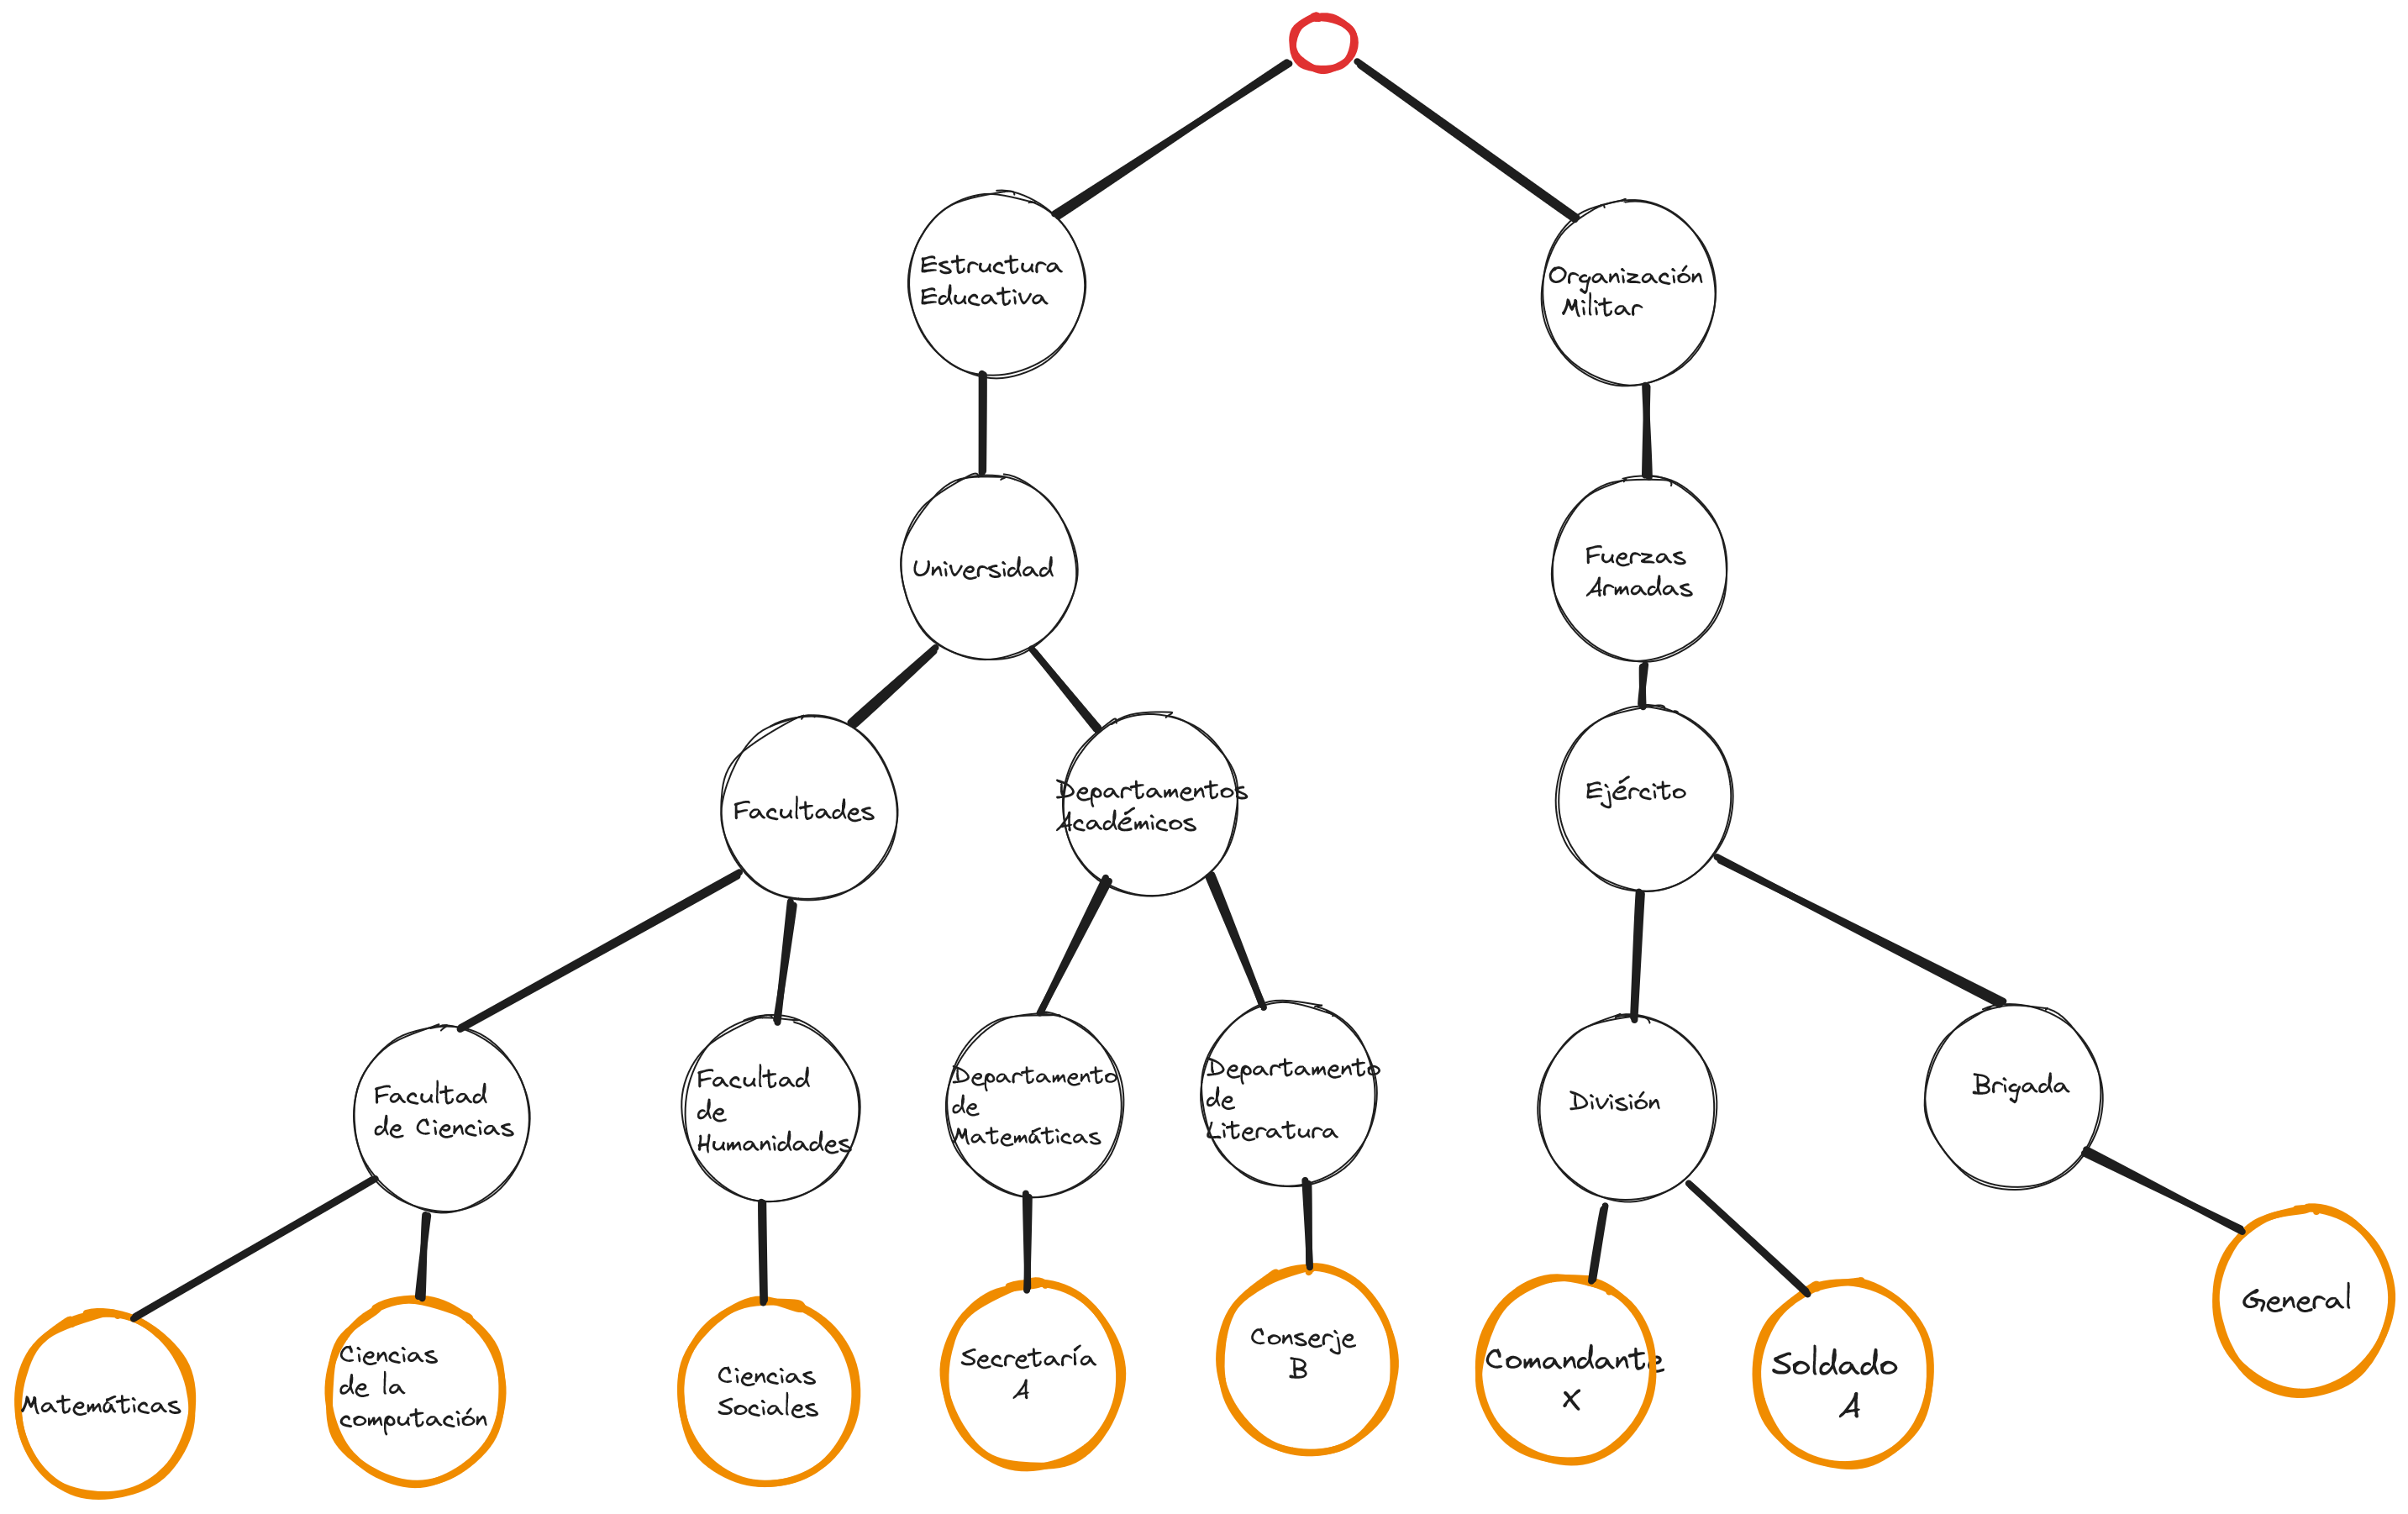
\includegraphics[width=14cm]{Arbol.png}}}
    \color{black}
    \label{fig:12}
\end{figure}

No dibujó los números de cuenta en su diagrama para ahorrar espacio pero cada nodo tiene su número de cuenta. Ahora con ese árbol solo tiene que hacer un recorrido DFS hasta llegar a las hojas para obtener las cuentas de detalle y construir la tabla anterior.

El problema es que Urrutia olvido casi todo su conocimiento de su curso de estructuras de datos de segundo semestre, pero seguramente tu no, así que te pedimos que le ayudes a Urrutia dandole el algoritmo "Inserta" para construir este árbol N-ario, es decir cada nodo puede tener uno o varios hijos, consideraciones a tomar en cuenta es que el nodo raíz es un nodo maestro que no almacena información pero sostiene a los nodos que si la tienen.

Se espera usar tu algoritmo "Inserta" para ir insertando las filas de las tablas iniciales uno por uno en orden jerarquico en forma de nodos, los nodos almacenan los nombres de cuenta y las llaves se basan en los números cuenta separados por un guión pero no necesariamente tienen que ser exactamente iguales.

Hints: Observa como los números de cuenta son grupos separados por guiones, para pasar de un nivel de jerarquía mayor a uno menor se conserva el prefijo y se modifica el sufijo. \\ ¿Que pasaría si por ejemplo convertimos "1-00-00-00-0000" a "1" y "1-01-00-00-0000" a "1-1"? ¿Como sabemos que "1-1" es un número de cuenta de menor jerarquía que "1"? (2 puntos)
\end{enumerate}

\end{document}

